%%%%%%%%%%%%

\section{A}

\begin{figure}[H]
	\centering
	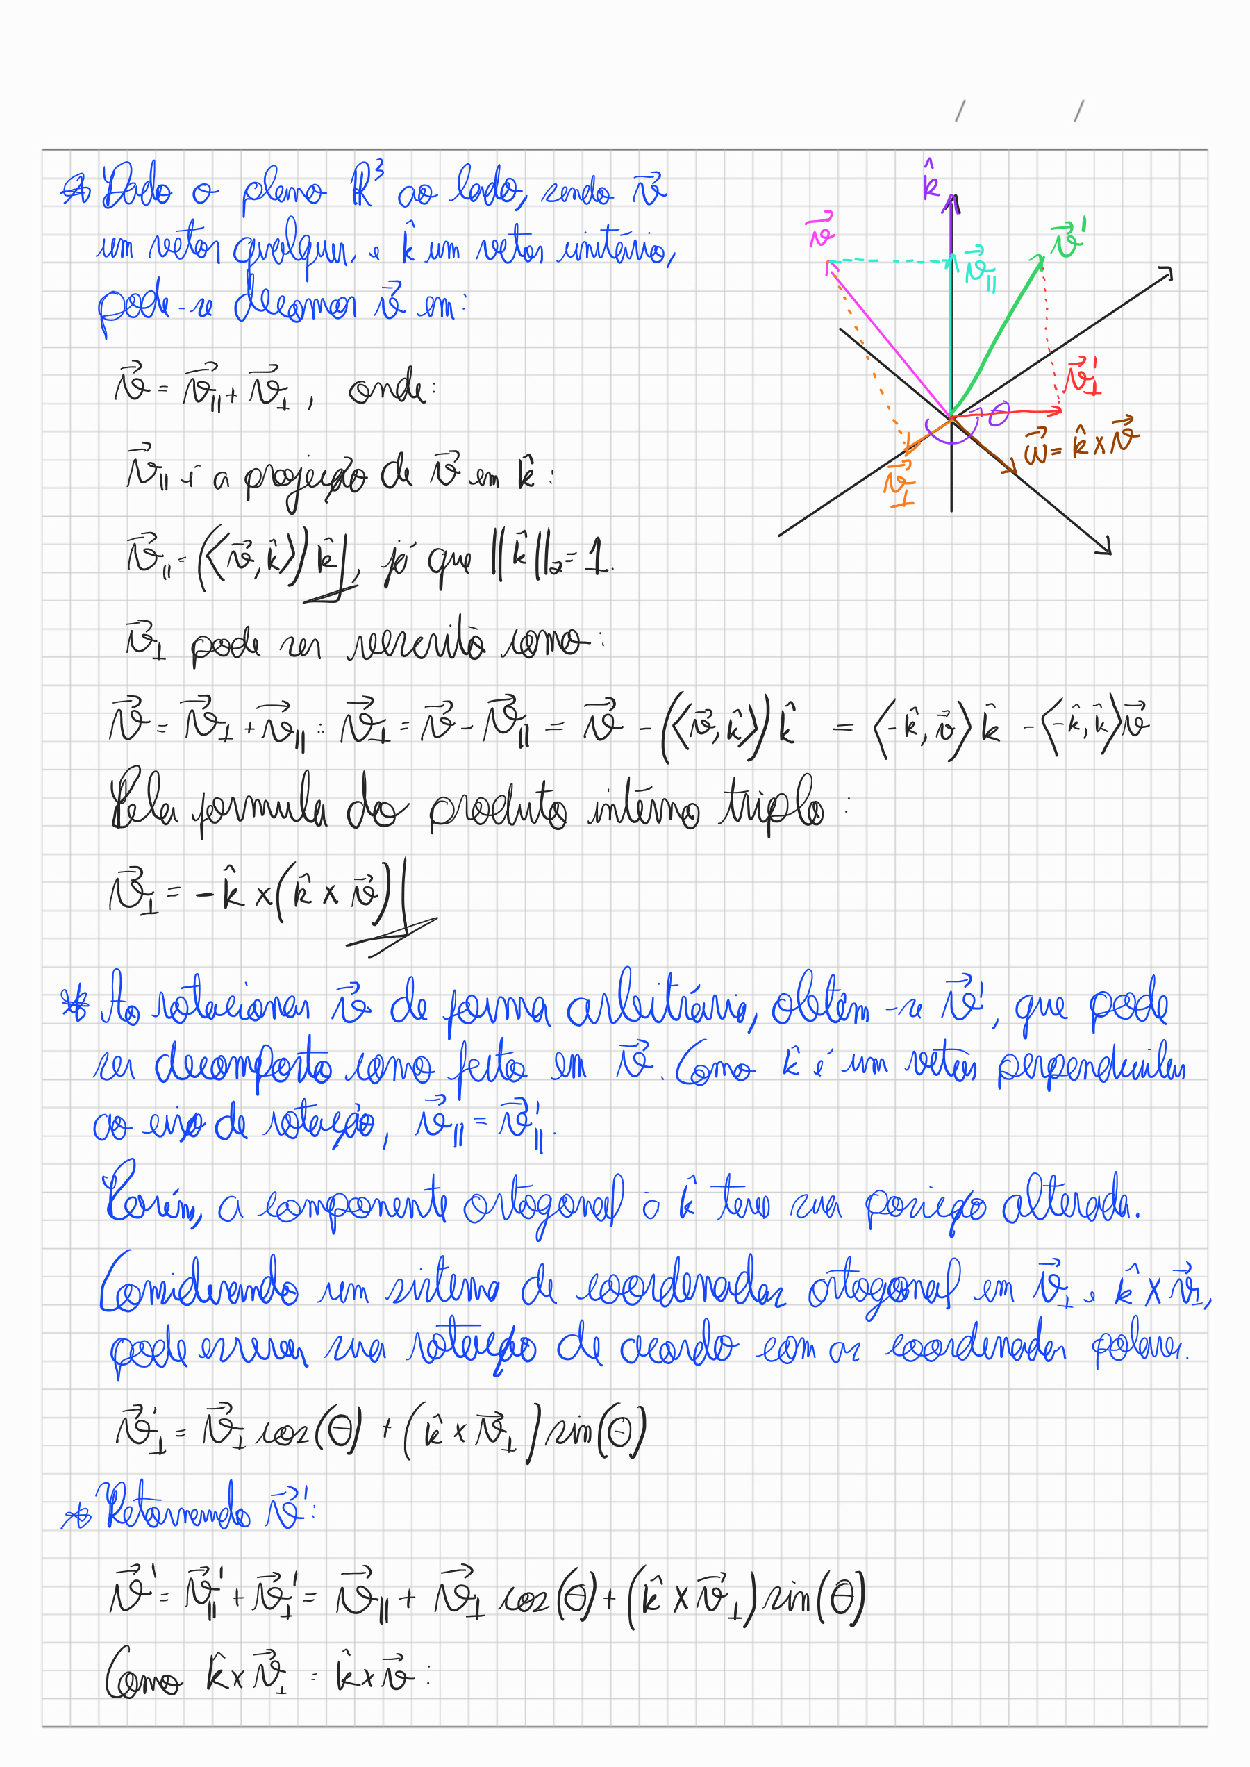
\includegraphics[width=0.99\linewidth]{img/A/RodriguesRotation-1}
	\label{fig:rodriguesrotation-2}
\end{figure}

\begin{figure}[H]
	\centering
	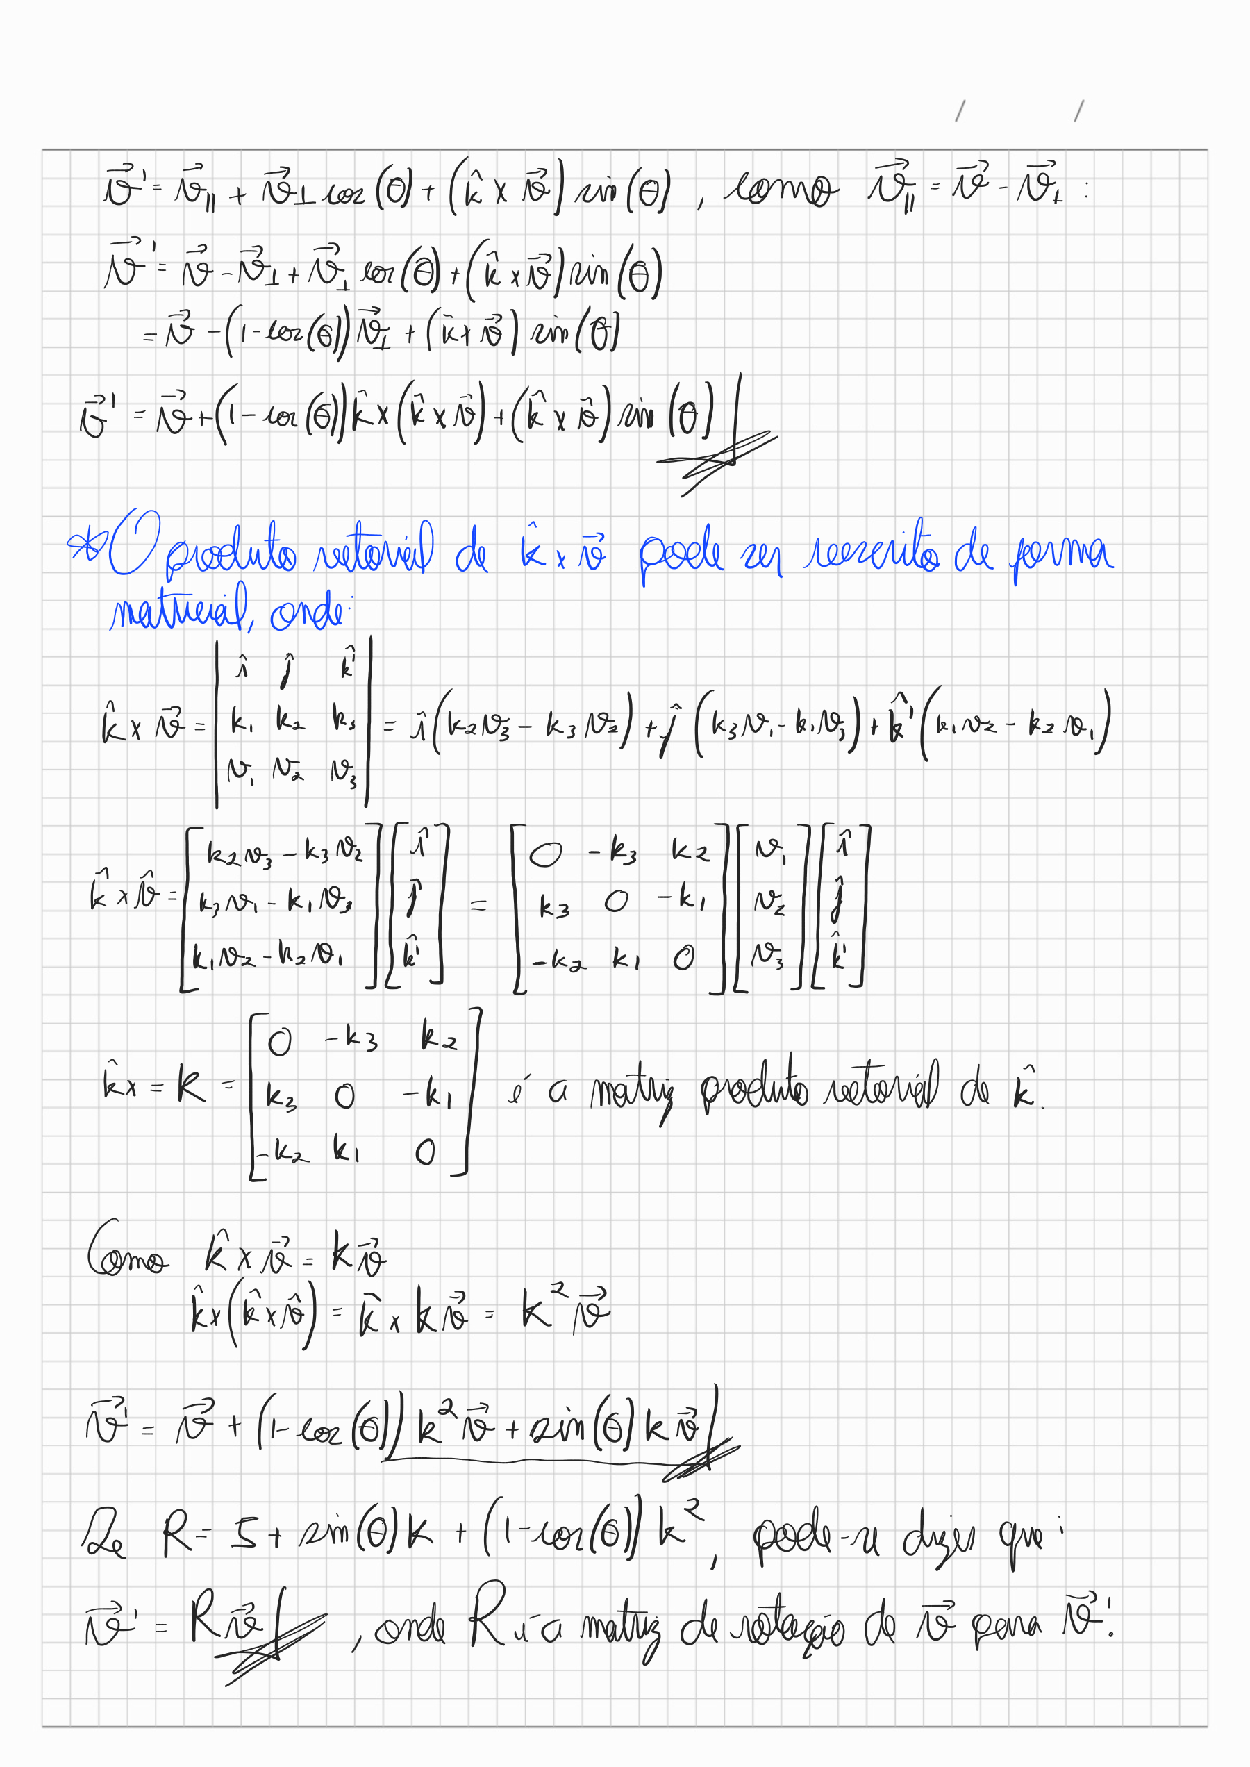
\includegraphics[width=1\linewidth]{img/A/RodriguesRotation-2}
	\label{fig:rodriguesrotation-3}
\end{figure}

\begin{figure}[H]
	\centering
	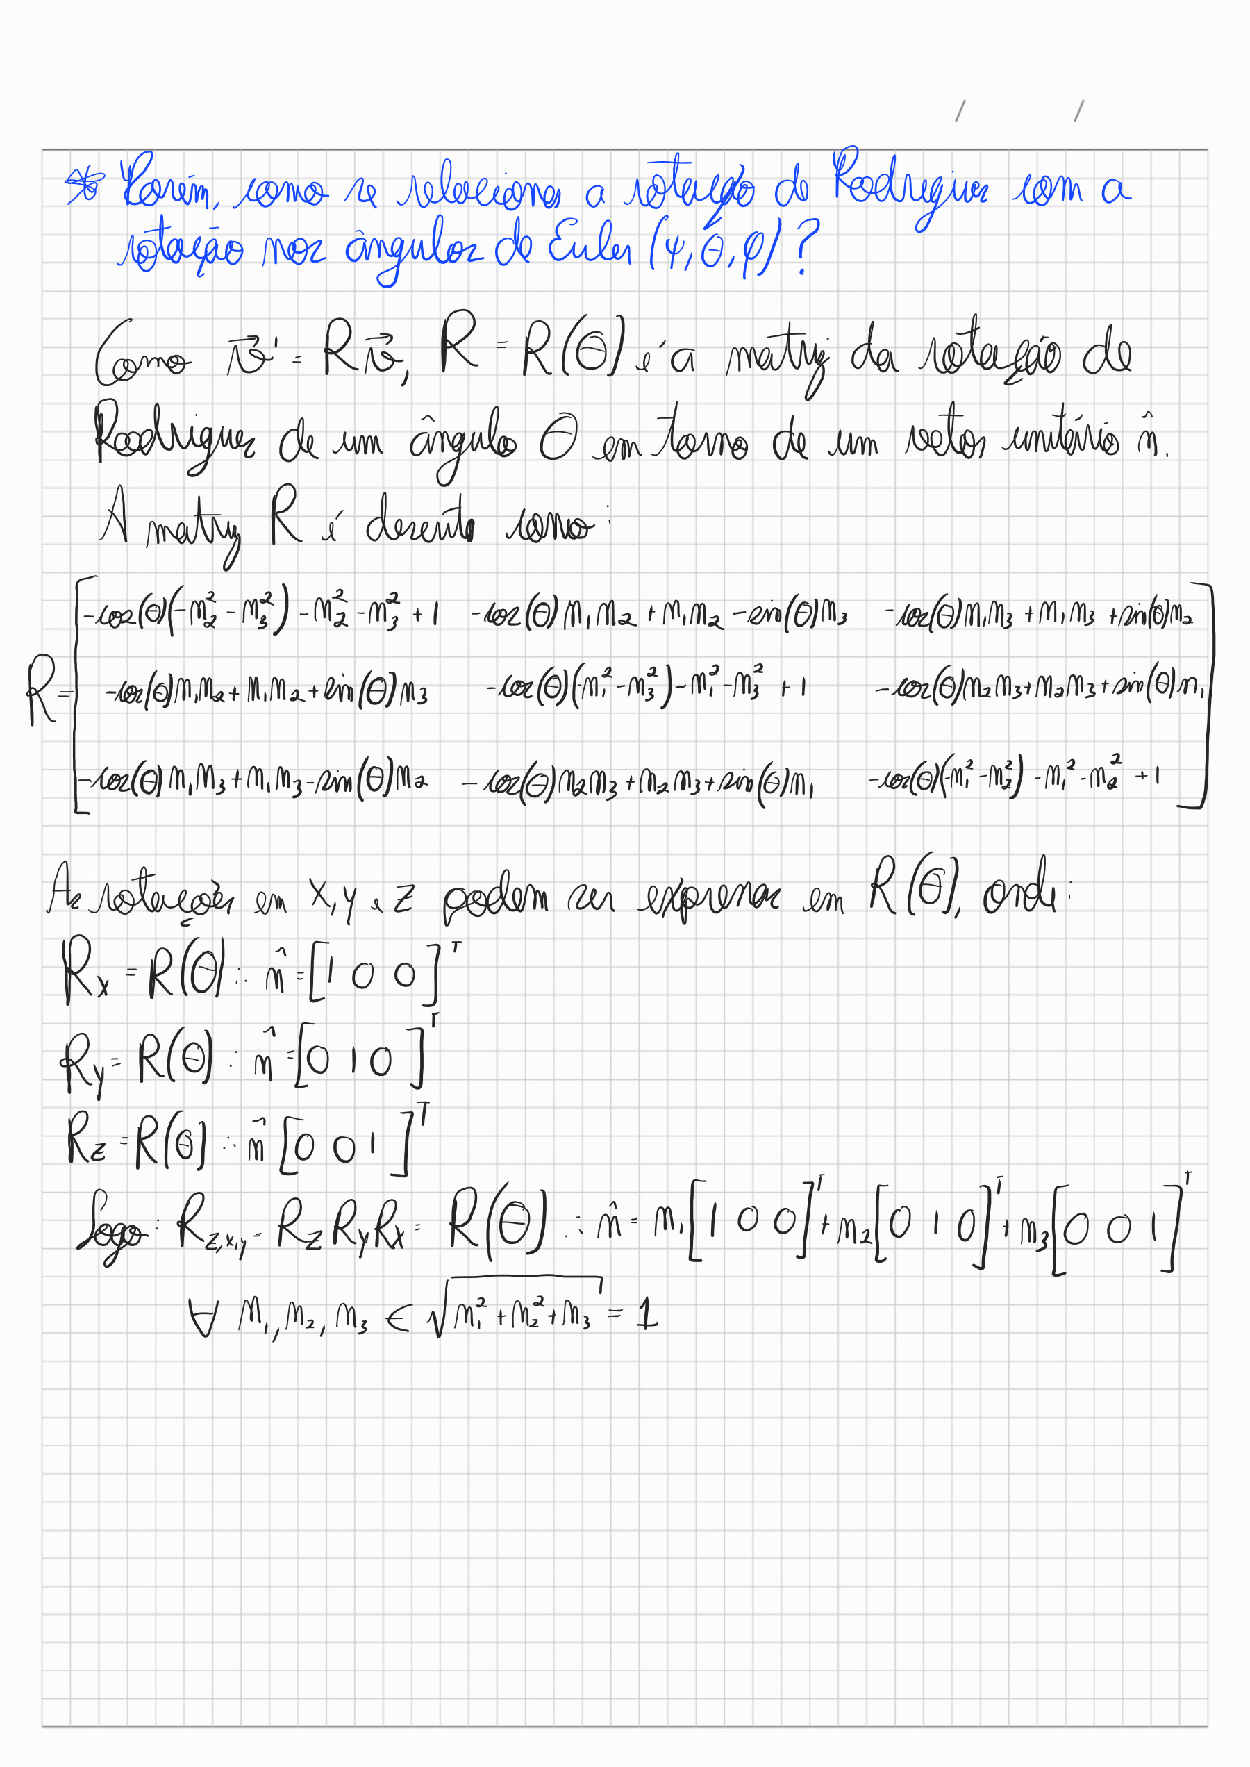
\includegraphics[width=1\linewidth]{img/A/RodriguesRotation-3}
	\label{fig:rodriguesrotation-4}
\end{figure}

\begin{figure}[H]
	\centering
	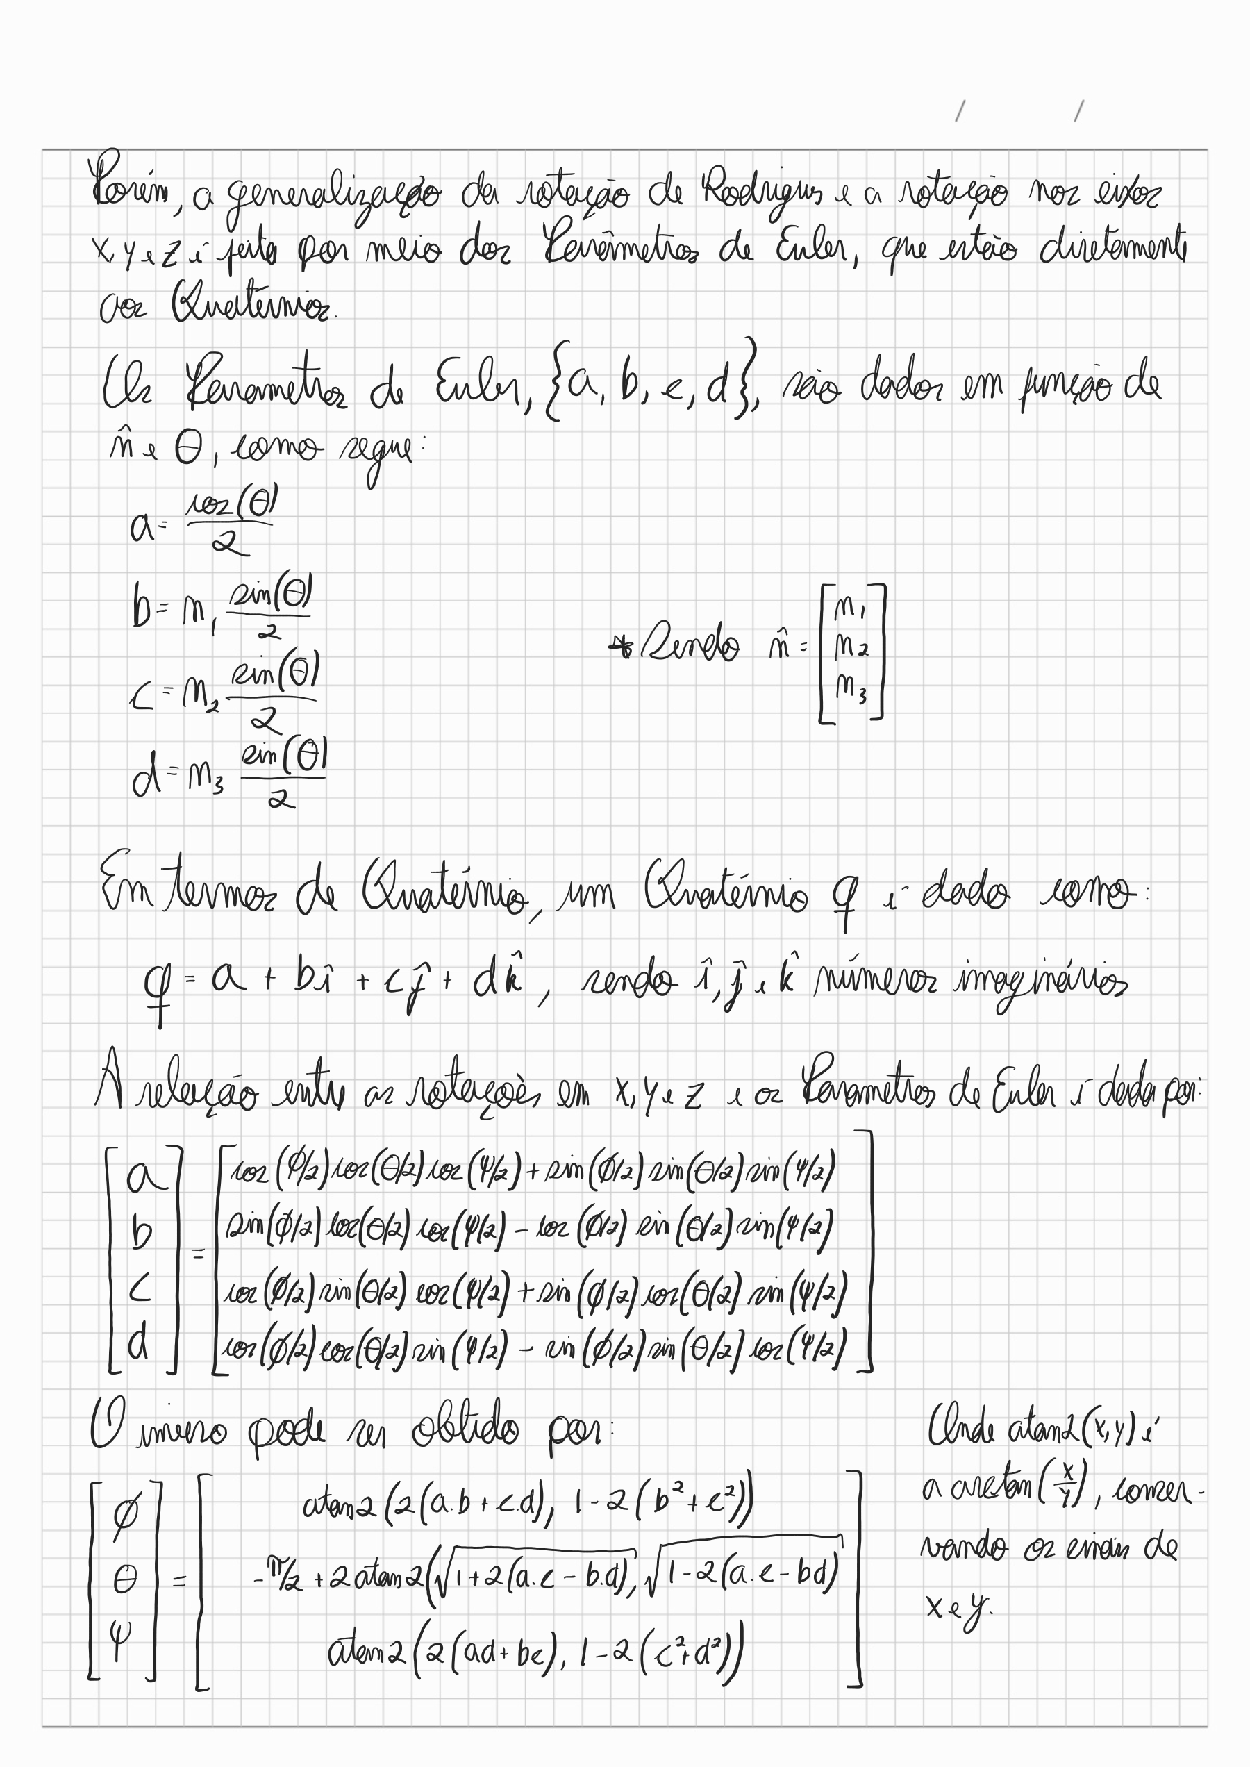
\includegraphics[width=1\linewidth]{img/A/RodriguesRotation-4}
	\label{fig:rodriguesrotation-1}
\end{figure}



%%%%%%%%%%%%%%%%%%%%%%%%%%%
\section{B}

Sendo um ponto descrito no sistema de coordenadas \{1\}, dado por $\+p_1 = \left[ 1 \ 2 \ 3 \right]^T$ (m), o mesmo pode ser escrito em outro sistema de referências desde que se saiba qual é a translação e a rotação entre esses dois sistemas de referência.

Uma vez que a translação entre o sistema de referência \{1\} e \{2\} é dado por $\+t = \left[1 \ 2 \ 15 \right]^T$, e a rotação $\{\phi, \theta, \psi\} = \{2^\circ, 1^\circ, 2^\circ\}$, pode-se escrever o ponto no \textit{frame} \{2\} conforme \eqref{eq:transform}.

\begin{equation}\label{eq:transform}
	\+p_2 = \+R(\{\phi, \theta, \psi\})\+p_1 + \+t
\end{equation}

Onde:

\begin{equation}\label{key}
	 \+R(\{\phi, \theta, \psi\}) = \+R(\psi) \+R(\theta)  \+R(\phi)
\end{equation}

A transformação de referencial foi implementada por meio da classe \texttt{tf}, descrita abaixo.

\begin{lstlisting}[language=python]
class tf:
	def __init__(self, x, y, z, phi, theta, psi):
		self.x = x
		self.y = y
		self.z = z 
		self.phi = np.deg2rad(phi)
		self.theta = np.deg2rad(theta)
		self.psi = np.deg2rad(psi)
		
		self.t = np.array([[x, y ,z]]).T

	def getPoint(self,p1):
		Rx = np.array([[1, 0, 0], [0, np.cos(self.psi), np.sin(self.psi)], [0, -np.sin(self.psi), np.cos(self.psi)]])
		Ry = np.array([[np.cos(self.theta), 0, -np.sin(self.theta)], [0, 1, 0], [np.sin(self.theta), 0, np.cos(self.theta)]])
		Rz = np.array([[np.cos(self.phi), np.sin(self.phi), 0], [-np.sin(self.phi), np.cos(self.phi), 0], [0, 0, 1]])
		R = np.matmul(Rz,np.matmul(Ry,Rx))
		
		p2 = np.matmul(R,p1) + self.t
		return p2
\end{lstlisting}

Executando a transformação, obteve-se a representação \eqref{eq:p2} do ponto $\+p_1$ no referencial \{2\}.

\begin{equation}\label{eq:p2}
	\+p_2 = \begin{bmatrix}
		2.02157298 \\
		4.06908819\\
		17.94537989
	\end{bmatrix}
\end{equation}
%%%%%%%%%%%%%%%%%%%%%%%%%%%
\section{C}

Dados as representações do ponto $\+p_1$ e $\+p_2$, ambos podem ser representados nas coordenadas da projeção desses pontos no plano da imagem, por meio dos pontos $\+q_1$ e $\+q_2$. A transformação é dada por \eqref{eq:proj}.

\begin{equation}\label{eq:proj}
	\+q = \+p\frac{f}{p_z}
\end{equation}

Sendo $f = 0,05$ m, têm-se que:

\begin{align}
	\+q_1 &= \begin{bmatrix}
		0.01667 \\
		0.03333 \\
		0.05 \\
	\end{bmatrix} \text{ (m)} \\
	\+q_2 &= \begin{bmatrix}
	0.00563\\
	0.01134\\
	0.05      \\
	\end{bmatrix} \text{ (m)} 
\end{align}

%%%%%%%%%%%%%%%%%%%%%%%%%%%
\section{D}

A projeção no plano da imagem é representadas em unidades métricas, não sendo essa a representação final da imagem capturada em termos da imagem em si. A projeção da imagem pode ser transformada para coordenadas de imagem, por meio de \eqref{eq:image}.

\begin{equation}\label{eq:image}
	\widehat{\+q} = \texttt{floor}\left(\frac{1}{f}\+A\+q\right)
\end{equation}

Sendo a matriz de parâmetros intrínsecos ($\+A$) dada por \eqref{eq:A}.

\begin{equation}\label{eq:A}
	\+A = \begin{bmatrix}
		fs_x & 0 & u_0 \\
		0 & fs_y & v_0\\
		0 & 0 & 1
	\end{bmatrix}
\end{equation}

Onde tem-se que:

\begin{align}
	s_x &= \frac{M}{L_x} \\
	s_y &= \frac{N}{L_y} \\
	u_0 &= 0 \\
	v_0 &= 0 
\end{align}

Dessa forma, obtém-se $\widehat{\+q}_1$ e $\widehat{\+q}_1$:

\begin{align}
	\widehat{\+q}_1 &= \texttt{floor}\left(\frac{1}{f}\+A\+q_1\right) = \begin{bmatrix}
		27\\
		69\\
		1
	\end{bmatrix}  \text{ (pixel)}\\
	\widehat{\+q}_2 &= \texttt{floor}\left(\frac{1}{f}\+A\+q_2\right)  = \begin{bmatrix}
		9\\
		23\\
		1
	\end{bmatrix}  \text{ (pixel)}
\end{align}

%%%%%%%%%%%%%%%%%%%%%%%%%%%
\section{E}

Relacionando o ponto no mundo com sua projeção no plano da imagem, como feito em \eqref{eq:pq}, pode-se substituir o ponto projetado para obter diretamente a coordenada do mundo em coordenadas de imagem, como em \eqref{eq:qqhat}.

Isolando $\+p$ em \eqref{eq:qqhat}, obtém-se em \eqref{eq:pqqhat} a transformação de reprojeção, do ponto em coordenadas de imagem para coordenadas do mundo.

\begin{equation}\label{eq:pq}
	\+q = \frac{f}{p_z}\+p 
\end{equation}

\begin{equation}\label{eq:qqhat}
	\widehat{\+q} = \frac{1}{f}\+A \+q  = \frac{1}{f}\+A\frac{f}{p_z}\+p  = \frac{1}{p_z}\+A\+p 
\end{equation}

\begin{equation}\label{eq:pqqhat}
	\widehat{\+p} = \+A^{-1}\widehat{\+q}p_z
\end{equation}

Sendo $\widehat{\+p}$ o ponto reprojetado.

Dessa forma, foi possível reprojetar os pontos $\+p_1$ e $\+p_2$, obtendo os resultados abaixo:

\begin{equation}\label{eq:repp1}
	\widehat{\+p}_1 = \+A^{-1}\widehat{\+q_1}p_{1_z} = \begin{bmatrix}
		0.972\\
		  1.987\\
		   3
	\end{bmatrix}
\end{equation}

\begin{equation}\label{eq:repp1}
	\widehat{\+p}_2 = \+A^{-1}\widehat{\+q_2}p_{2_z} = \begin{bmatrix}
	1.938 \\
	 3.962 \\
	 17.945
\end{bmatrix}
\end{equation}

O erro de reprojeção foi calculado com base na média da distância euclidiana do vetor erro de reprojeção, dendo dado por \eqref{eq:errormean}.

\begin{equation}\label{eq:errormean}
	e = \frac{1}{N}\sum_{i=1}^{N}||\+{e_i}||_2 = \frac{1}{N}\sum_{i=1}^{N}||\+p_i - \widehat{\+p_i}||_2
\end{equation}

Para os pontos recuperados, o erro médio foi de 0,083.
